\documentclass[12pt]{article}

%%%% packages and definitions (optional)
\usepackage{graphicx} % allows inclusion of graphics
\usepackage{graphics}
\usepackage{placeins}
\usepackage{booktabs} % nice rules (thick lines) for tables
\usepackage{microtype} % improves typography for PDF
\usepackage{xspace}
\usepackage[hidelinks]{hyperref}
\usepackage{xspace}
\usepackage{hhline}


\usepackage{pgfgantt}
\usepackage{rotating}
\usepackage[graphicx]{realboxes}
\usepackage{lscape}
\usepackage[margin=0.5in,landscape]{geometry}


\def\pgfcalendarweekdayletter#1{%  
 \ifcase#1M\or Tu\or W\or Tr\or F\or Sa\or Su\fi%  
}  
\usepackage{amsmath}

\usepackage{tabularx}
\newcolumntype{b}{>{\hsize=1.0\hsize}X}
\newcolumntype{s}{>{\hsize=.5\hsize}X}
\newcolumntype{m}{>{\hsize=.75\hsize}X}

\newcommand{\SN}{S$_N$}
\renewcommand{\vec}[1]{\bm{#1}} %vector is bold italic
\newcommand{\vd}{\bm{\cdot}} % slightly bold vector dot
\newcommand{\grad}{\vec{\nabla}} % gradient
\newcommand{\ud}{\mathop{}\!\mathrm{d}} % upright derivative symbol
\newcommand{\Cyclus}{\textsc{Cyclus}\xspace}%
\graphicspath{ {images/} }
\usepackage[affil-it]{authblk}
\usepackage[numbers]{natbib}
\usepackage{notoccite}
\usepackage{tikz}
\usetikzlibrary{positioning, arrows, decorations, shapes }
\usepackage{cleveref}

\usepackage{datatool}
\usepackage[acronym,toc]{glossaries}
%\newacronym{<++>}{<++>}{<++>}
\newacronym[longplural={metric tons of heavy metal}]{MTHM}{MTHM}{metric ton of heavy metal}
\newacronym{ABM}{ABM}{agent-based modeling}
\newacronym{ACDIS}{ACDIS}{Program in Arms Control \& Domestic and International Security}
\newacronym{ADS}{ADS}{Accelerator-Driven Systems}
\newacronym{AHTR}{AHTR}{Advanced High Temperature Reactor}
\newacronym{ANDRA}{ANDRA}{Agence Nationale pour la gestion des D\'echets RAdioactifs, the French National Agency for Radioactive Waste Management}
\newacronym{ANL}{ANL}{Argonne National Laboratory}
\newacronym{ANS}{ANS}{American Nuclear Society}
\newacronym{API}{API}{application programming interface}
\newacronym{ARE}{ARE}{Aircraft Reactor Experiment}
\newacronym{ARFC}{ARFC}{Advanced Reactors and Fuel Cycles}
\newacronym{ASME}{ASME}{American Society of Mechanical Engineers}
\newacronym{ATWS}{ATWS}{Anticipated Transient Without Scram}
\newacronym{BDBE}{BDBE}{Beyond Design Basis Event}
\newacronym{BIDS}{BIDS}{Berkeley Institute for Data Science}
\newacronym{BWR}{BWR}{Boiling Water Reactor}
\newacronym{CAFCA}{CAFCA}{ Code for Advanced Fuel Cycles Assessment }
\newacronym{CDTN}{CDTN}{Centro de Desenvolvimento da Tecnologia Nuclear}
\newacronym{CEA}{CEA}{Commissariat \`a l'\'Energie Atomique et aux \'Energies Alternatives}
\newacronym{CI}{CI}{continuous integration}
\newacronym{CNEN}{CNEN}{Comiss\~{a}o Nacional de Energia Nuclear}
\newacronym{CNERG}{CNERG}{Computational Nuclear Engineering Research Group}
\newacronym{COSI}{COSI}{Commelini-Sicard}
\newacronym{COTS}{COTS}{commercial, off-the-shelf}
\newacronym{CSNF}{CSNF}{commercial spent nuclear fuel}
\newacronym{CTAH}{CTAHs}{Coiled Tube Air Heaters}
\newacronym{CUBIT}{CUBIT}{CUBIT Geometry and Mesh Generation Toolkit}
\newacronym{CURIE}{CURIE}{Centralized Used Fuel Resource for Information Exchange}
\newacronym{DAG}{DAG}{directed acyclic graph}
\newacronym{DANESS}{DANESS}{Dynamic Analysis of Nuclear Energy System Strategies}
\newacronym{DBE}{DBE}{Design Basis Event}
\newacronym{DESAE}{DESAE}{Dynamic Analysis of Nuclear Energy Systems Strategies}
\newacronym{DHS}{DHS}{Department of Homeland Security}
\newacronym{DOE}{DOE}{Department of Energy}
\newacronym{DRACS}{DRACS}{Direct Reactor Auxiliary Cooling System}
\newacronym{DRE}{DRE}{dynamic resource exchange}
\newacronym{DSNF}{DSNF}{DOE spent nuclear fuel}
\newacronym{DYMOND}{DYMOND}{Dynamic Model of Nuclear Development }
\newacronym{EBS}{EBS}{Engineered Barrier System}
\newacronym{EDF}{EDF}{Électricité de France}
\newacronym{EDZ}{EDZ}{Excavation Disturbed Zone}
\newacronym{EIA}{EIA}{U.S. Energy Information Administration}
\newacronym{EPA}{EPA}{Environmental Protection Agency}
\newacronym{EPR}{EPR}{European Pressurized Reactor}
\newacronym{EP}{EP}{Engineering Physics}
\newacronym{EU}{EU}{European Union}
\newacronym{FCO}{FCO}{Fuel Cycle Options}
\newacronym{FCT}{FCT}{Fuel Cycle Technology}
\newacronym{FEHM}{FEHM}{Finite Element Heat and Mass Transfer}
\newacronym{FEPs}{FEPs}{Features, Events, and Processes}
\newacronym{FHR}{FHR}{Fluoride-Salt-Cooled High-Temperature Reactor}
\newacronym{FLiBe}{FLiBe}{Fluoride-Lithium-Beryllium}
\newacronym{FP}{FP}{Fission Products}
\newacronym{GDSE}{GDSE}{Generic Disposal System Environment}
\newacronym{GDSM}{GDSM}{Generic Disposal System Model}
\newacronym{GENIUSv1}{GENIUSv1}{Global Evaluation of Nuclear Infrastructure Utilization Scenarios, Version 1}
\newacronym{GENIUSv2}{GENIUSv2}{Global Evaluation of Nuclear Infrastructure Utilization Scenarios, Version 2}
\newacronym{GENIUS}{GENIUS}{Global Evaluation of Nuclear Infrastructure Utilization Scenarios}
\newacronym{GPAM}{GPAM}{Generic Performance Assessment Model}
\newacronym{GRSAC}{GRSAC}{Graphite Reactor Severe Accident Code}
\newacronym{GUI}{GUI}{graphical user interface}
\newacronym{HLW}{HLW}{high level waste}
\newacronym{HPC}{HPC}{high-performance computing}
\newacronym{HTC}{HTC}{high-throughput computing}
\newacronym{HTGR}{HTGR}{High Temperature Gas-Cooled Reactor}
\newacronym{IAEA}{IAEA}{International Atomic Energy Agency}
\newacronym{IEMA}{IEMA}{Illinois Emergency Mangament Agency}
\newacronym{IHLRWM}{IHLRWM}{International High Level Radioactive Waste Management}
\newacronym{INL}{INL}{Idaho National Laboratory}
\newacronym{IPRR1}{IRP-R1}{Instituto de Pesquisas Radioativas Reator 1}
\newacronym{IRP}{IRP}{Integrated Research Project}
\newacronym{ISFSI}{ISFSI}{Independent Spent Fuel Storage Installation}
\newacronym{ISRG}{ISRG}{Independent Student Research Group}
\newacronym{JFNK}{JFNK}{Jacobian-Free Newton Krylov}
\newacronym{LANL}{LANL}{Los Alamos National Laboratory}
\newacronym{LBNL}{LBNL}{Lawrence Berkeley National Laboratory}
\newacronym{LCOE}{LCOE}{levelized cost of electricity}
\newacronym{LDRD}{LDRD}{laboratory directed research and development}
\newacronym{LFR}{LFR}{Lead-Cooled Fast Reactor}
\newacronym{LLNL}{LLNL}{Lawrence Livermore National Laboratory}
\newacronym{LMFBR}{LMFBR}{Liquid Metal Fast Breeder Reactor}
\newacronym{LOFC}{LOFC}{Loss of Forced Cooling}
\newacronym{LOHS}{LOHS}{Loss of Heat Sink}
\newacronym{LOLA}{LOLA}{Loss of Large Area}
\newacronym{LP}{LP}{linear program}
\newacronym{LWR}{LWR}{Light Water Reactor}
\newacronym{MAGNOX}{MAGNOX}{Magnesium Alloy Graphie Moderated Gas Cooled Uranium Oxide Reactor}
\newacronym{MA}{MA}{minor actinide}
\newacronym{MCNP}{MCNP}{Monte Carlo N-Particle code}
\newacronym{MILP}{MILP}{mixed-integer linear program}
\newacronym{MIT}{MIT}{the Massachusetts Institute of Technology}
\newacronym{MOAB}{MOAB}{Mesh-Oriented datABase}
\newacronym{MOOSE}{MOOSE}{Multiphysics Object-Oriented Simulation Environment}
\newacronym{MOX}{MOX}{Mixed Oxide Fuel}
\newacronym{MSBR}{MSBR}{Molten Salt Breeder Reactor}
\newacronym{MSRE}{MSRE}{Molten Salt Reactor Experiment}
\newacronym{MSR}{MSR}{Molten Salt Reactor}
\newacronym{NAGRA}{NAGRA}{National Cooperative for the Disposal of Radioactive Waste}
\newacronym{NEAMS}{NEAMS}{Nuclear Engineering Advanced Modeling and Simulation}
\newacronym{NEUP}{NEUP}{Nuclear Energy University Programs}
\newacronym{NFCSim}{NFCSim}{Nuclear Fuel Cycle Simulator}
\newacronym{NGNP}{NGNP}{Next Generation Nuclear Plant}
\newacronym{NMWPC}{NMWPC}{Nuclear MW Per Capita}
\newacronym{NNSA}{NNSA}{National Nuclear Security Administration}
\newacronym{NPRE}{NPRE}{Department of Nuclear, Plasma, and Radiological Engineering}
\newacronym{NQA1}{NQA-1}{Nuclear Quality Assurance - 1}
\newacronym{NRC}{NRC}{Nuclear Regulatory Commission}
\newacronym{NSF}{NSF}{National Science Foundation}
\newacronym{NSSC}{NSSC}{Nuclear Science and Security Consortium}
\newacronym{NUWASTE}{NUWASTE}{Nuclear Waste Assessment System for Technical Evaluation}
\newacronym{NWF}{NWF}{Nuclear Waste Fund}
\newacronym{NWTRB}{NWTRB}{Nuclear Waste Technical Review Board}
\newacronym{OCRWM}{OCRWM}{Office of Civilian Radioactive Waste Management}
\newacronym{ORION}{ORION}{ORION}
\newacronym{ORNL}{ORNL}{Oak Ridge National Laboratory}
\newacronym{PARCS}{PARCS}{Purdue Advanced Reactor Core Simulator}
\newacronym{PBAHTR}{PB-AHTR}{Pebble Bed Advanced High Temperature Reactor}
\newacronym{PBFHR}{PB-FHR}{Pebble-Bed Fluoride-Salt-Cooled High-Temperature Reactor}
\newacronym{PEI}{PEI}{Peak Environmental Impact}
\newacronym{PH}{PRONGHORN}{PRONGHORN}
\newacronym{PRA}{PRA}{probabilistic risk assessment}
\newacronym{PRIS}{PRIS}{Power Reactor Information System}
\newacronym{PRKE}{PRKE}{Point Reactor Kinetics Equations}
\newacronym{PSPG}{PSPG}{Pressure-Stabilizing/Petrov-Galerkin}
\newacronym{PWAR}{PWAR}{Pratt and Whitney Aircraft Reactor}
\newacronym{PWR}{PWR}{Pressurized Water Reactor}
\newacronym{PyNE}{PyNE}{Python toolkit for Nuclear Engineering}
\newacronym{PyRK}{PyRK}{Python for Reactor Kinetics}
\newacronym{QA}{QA}{quality assurance}
\newacronym{RDD}{RD\&D}{Research Development and Demonstration}
\newacronym{RD}{R\&D}{Research and Development}
\newacronym{RELAP}{RELAP}{Reactor Excursion and Leak Analysis Program}
\newacronym{RIA}{RIA}{Reactivity Insertion Accident}
\newacronym{RIF}{RIF}{Region-Institution-Facility}
\newacronym{SFR}{SFR}{Sodium-Cooled Fast Reactor}
\newacronym{SINDAG}{SINDA{\textbackslash}G}{Systems Improved Numerical Differencing Analyzer $\backslash$ Gaski}
\newacronym{SKB}{SKB}{Svensk K\"{a}rnbr\"{a}nslehantering AB}
\newacronym{SNF}{SNF}{spent nuclear fuel}
\newacronym{SNL}{SNL}{Sandia National Laboratory}
\newacronym{STC}{STC}{specific temperature change}
\newacronym{SUPG}{SUPG}{Streamline-Upwind/Petrov-Galerkin}
\newacronym{SWF}{SWF}{Separations and Waste Forms}
\newacronym{SWU}{SWU}{Separative Work Unit}
\newacronym{TRIGA}{TRIGA}{Training Research Isotope General Atomic}
\newacronym{TRISO}{TRISO}{Tristructural Isotropic}
\newacronym{TSM}{TSM}{Total System Model}
\newacronym{TSPA}{TSPA}{Total System Performance Assessment for the Yucca Mountain License Application}
\newacronym{ThOX}{ThOX}{thorium oxide}
\newacronym{UFD}{UFD}{Used Fuel Disposition}
\newacronym{UML}{UML}{Unified Modeling Language}
\newacronym{UNF}{UNF}{Used Nuclear Fuel}
\newacronym{UOX}{UOX}{Uranium Oxide Fuel}
\newacronym{UQ}{UQ}{uncertainty quantification}
\newacronym{US}{US}{United States}
\newacronym{UW}{UW}{University of Wisconsin}
\newacronym{VISION}{VISION}{the Verifiable Fuel Cycle Simulation Model}
\newacronym{VVER}{VVER}{Voda-Vodyanoi Energetichesky Reaktor (Russian Pressurized Water Reactor)}
\newacronym{VV}{V\&V}{verification and validation}
\newacronym{WIPP}{WIPP}{Waste Isolation Pilot Plant}
\newacronym{YMR}{YMR}{Yucca Mountain Repository Site}

	
\makeglossaries

\title{Probabilistic Risk Assessment of Mined Nuclear Spent Fuel Repositories }
\author{Jin Whan Bae}
\affil{Dept. of Nuclear, Plasma, and Radiological Engineering, University of Illinois at Urbana-Champaign
		  Urbana, IL}
\date{}                     %% if you don't need date to appear
\setcounter{Maxaffil}{0}
\renewcommand\Affilfont{\itshape\small}
%%%%%%%%%%%%%%actual words%%%%%%%%%%%%%%%%%%%%%%%%%%%%%%%%%%%%%%%%%%%%%%%%%%%%5


\begin{document}
\maketitle

\section{Abstract}
\gls{UNF} repositories, given the high decay heat and radioactivity
of \glspl{UNF}, requires careful engineering. The current plan is
to design a repository that would contain the material for one million years.
Considering various events (failures) can occur in that time range,
the \gls{UNF} repository proposes an interesting subject for
\gls{PRA}. In this report, the model repository design is after the 
\gls{YMR}, which is a mined repository in volcanic tuff.
Ultimate failure status can be defined in various ways, depending on the
extent of leakage during the one million years (leakage from canister
\textasciitilde exposure to nearest population).
A definitive exposure of failure criteria must be defined,
in order for a reasonable analysis.  

Given the expansive
time range, very little real data is available, which makes
most of the probability values a Bayesian, a `degree-of-confidence' value.
Other data can be derived from scientific data, such as 
corrosion and precipitation in the area, but would have to be extrapolated
with assumptions for the given time range.

The failure scenario would begin from the canister's arrival at the
site, namely, from the repackaging facility. The repackaging facility
would take out the individual assemblies from the transportation cask
and emplace the assemblies in a storage cask. There, the storage cask
would be moved to the repository to sit for a million years. 
Given the successful emplacement of the fuel canister, the canister
must corrode, or break, in order to expose the radioactive materials
inside. The exposed radioactive materials would be transported, through
various methods (person carrying it out, precipitation flow etc.)
to affect the population, causing the system to fail.


\section{Goal}
The goal of this project is to create a simplistic case study of the
\gls{YMR} with RISKMAN. Various aspects of the repository
will be modeled in different ways, from empirical failure point probability data,
distributions with uncertainty, and human failure models.

\section{Schedule}
\noindent\resizebox{\textwidth}{!}{
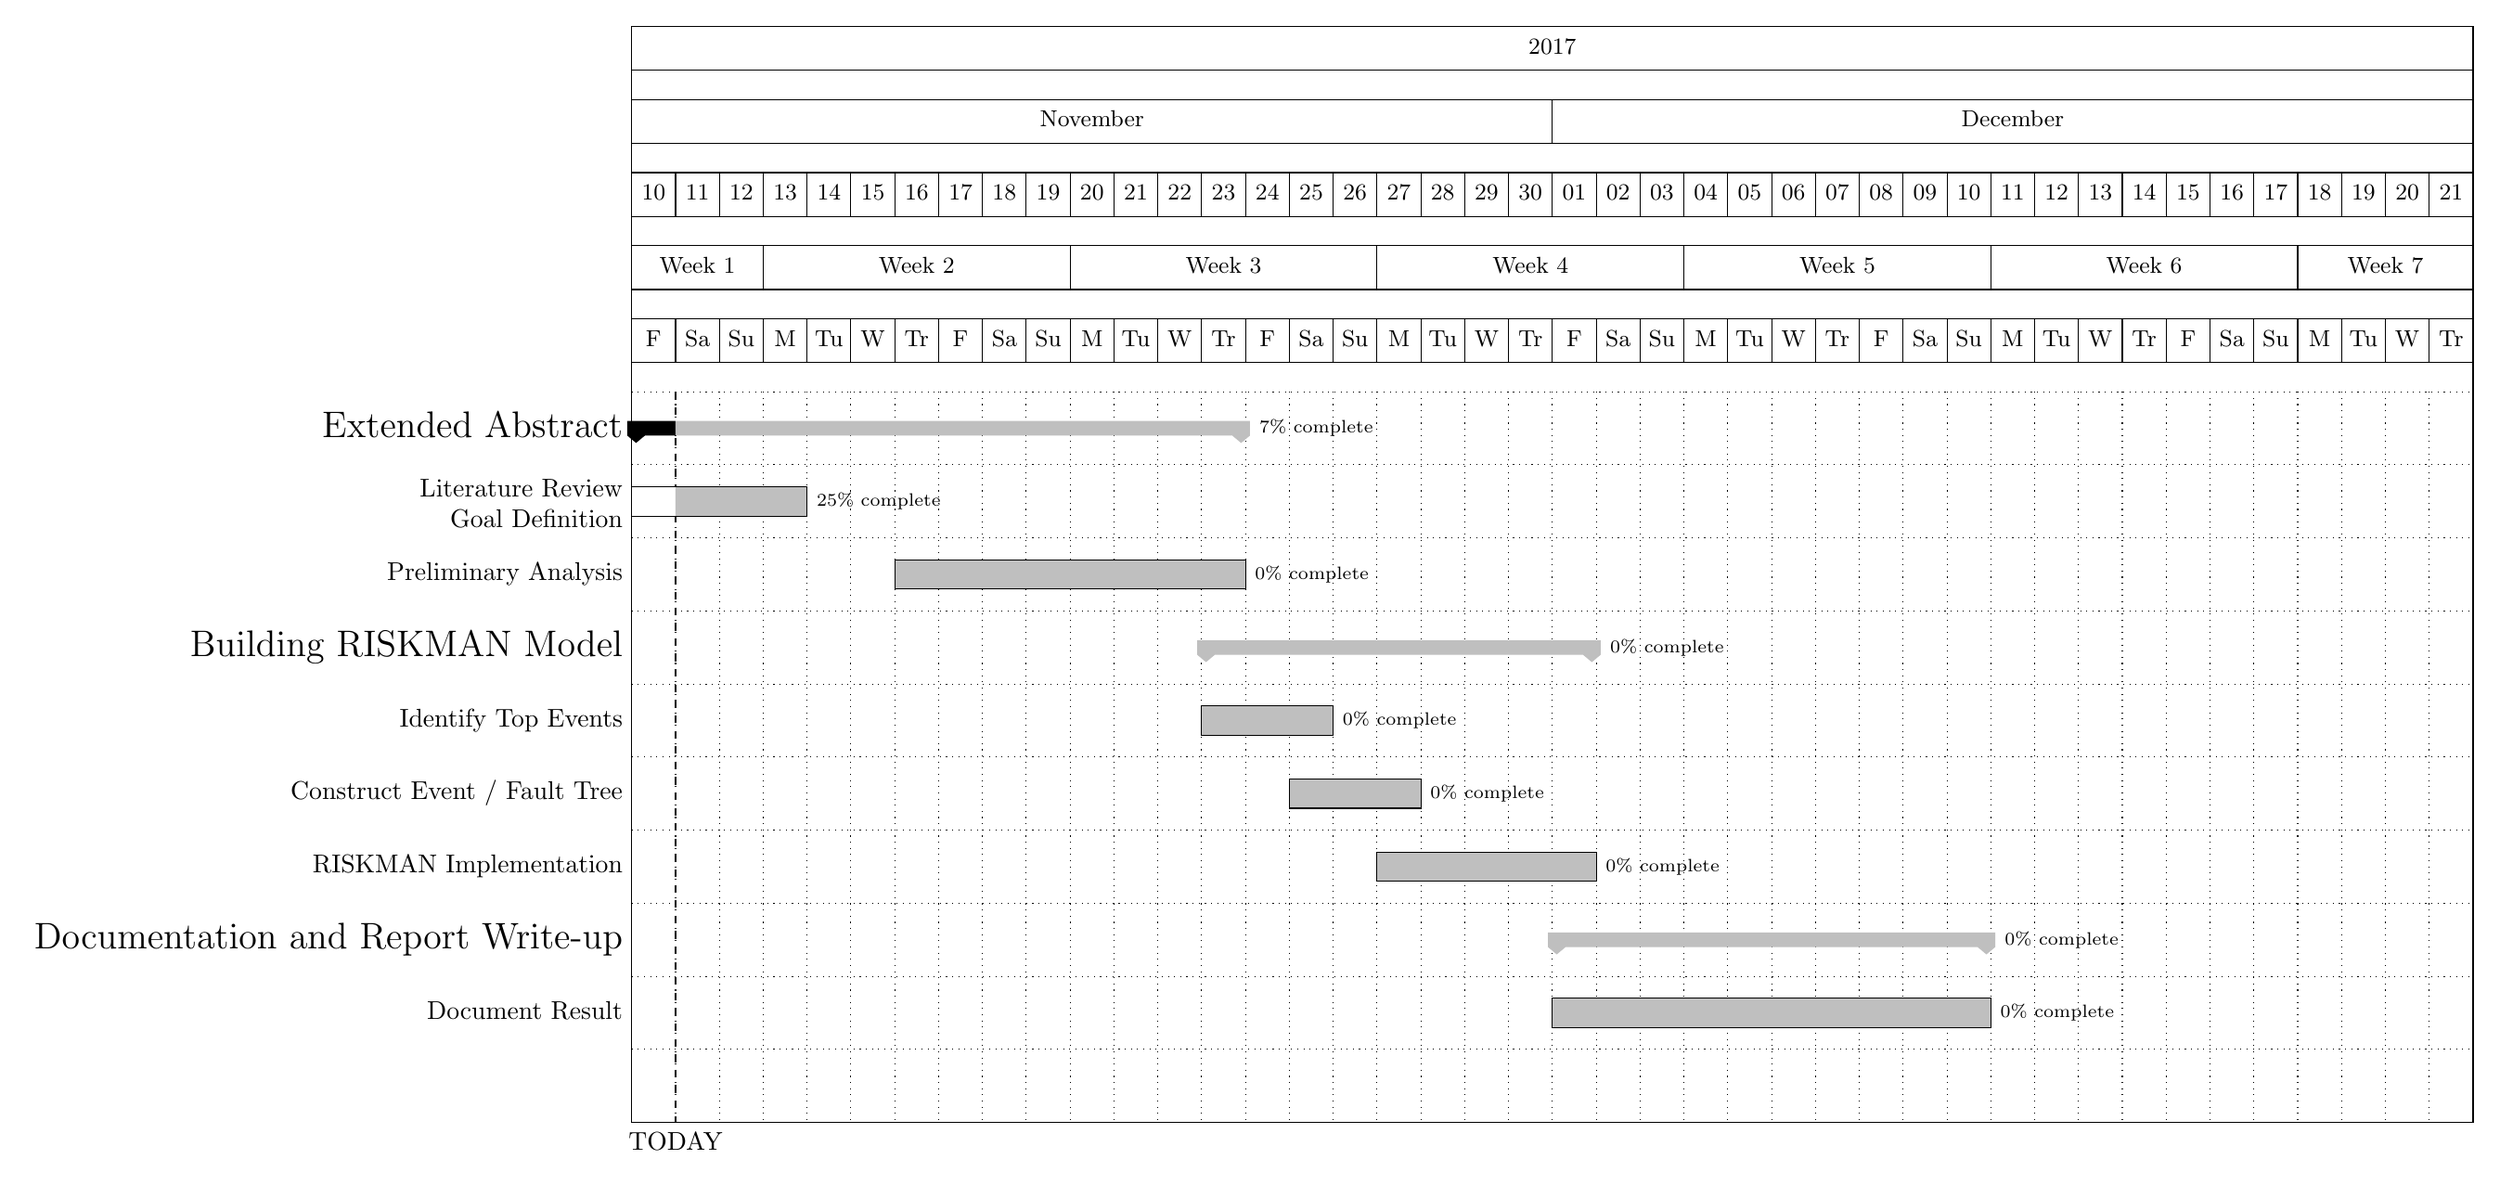
\begin{tikzpicture}[x=.5cm, y=1cm]
\begin{ganttchart}[
    hgrid,
    vgrid,
    group label font=\Large,
    progress=today,
    today=2017-11-10,
    x unit=6mm,
    newline shortcut=true,
    bar label node/.append style={align=right},
    time slot format=isodate
    ]{2017-11-10}{2017-12-21}
    \gantttitlecalendar{year, month=name, day, week=1, weekday=letter} \\
    
    \ganttgroup{Extended Abstract}{2017-11-10}{2017-11-23} \\
    \ganttbar{Literature Review \ganttalignnewline Goal Definition}{2017-11-10}{2017-11-13} \\
    \ganttbar{Preliminary Analysis}{2017-11-16}{2017-11-23} \\

    
    \ganttgroup{Building RISKMAN Model}{2017-11-23}{2017-12-01} \\
    \ganttbar{Identify Top Events}{2017-11-23}{2017-11-25}\\
    \ganttbar{Construct Event / Fault Tree}{2017-11-25}{2017-11-27} \\
    \ganttbar{RISKMAN Implementation}{2017-11-27}{2017-12-01} \\

    \ganttgroup{Documentation and Report Write-up}{2017-12-01}{2017-12-10}\\
    \ganttbar{Document Result}{2017-12-01}{2017-12-10} \\
    
    

    
\end{ganttchart}
\end{tikzpicture}
}


\section{Background}
\gls{YMR} has been studied thoroughly in hopes of finally
disposing the U.S. \gls{UNF} inventory. However, considering
that it is a large project involving highly radioactive material,
careful planning and analyses must be done. The reference design
is taken from various sources \cite{u.s._department_of_energy_office_of_civilian_radioactive_waste_management_national_2008, wilson_total-system_1994, rechard_evolution_2014}.
The RISKMAN model will attempt to capture various factors in the design.


\section{Literature Review}
System designs of the \gls{YMR} are listed extensively in literature \cite{u.s._department_of_energy_office_of_civilian_radioactive_waste_management_national_2008, wilson_total-system_1994, rechard_evolution_2014}, and contain multiple
iterations on the design. The basic design is as follows: the spent fuel assemblies
are repackaged in the waste package canister, and then placed underground,
underneath a drip shield. The canisters will remain there for up to millions of years,
surrounded by volcanic tuff.

Some prominent risk factors have also been identified. Volcanic hazards \cite{ho_risk_1992, smith_area_1990}
have been identified to be a long-term issue. Groundwater movement and transport of 
radioactive isotopes are another issue, in the case of canister breach \cite{robison_ground-water_1984, quade_fossil_1995}.  Canister reliability is another
identified risk factor \cite{whipple_can_1996, rutqvist_analysis_2003}.

Different aspects of risk analysis for nuclear waste repositories are published.
For systems where the future is hardly predictable, bayesian network analyses are 
suggested in \cite{lee_application_2006}. A method for sensitivity analysis
to rank important parameters are suggested in \cite{mohanty_cdf_2001}.


\section{Method}

From the literature review, a crude diagram of the \gls{YMR} system is drawn.
From the diagram, important subsystems are identified, with possible initiating
events that cause them to fail. The subsystems are then linked upon their dependence.
The initiating events and the related event trees are developed, along with the
fault tree of the events, if applicable. The probability of basic events or components
then would be modeled
appropriately, using various methods like point estimate or distributions.
The constructed system reliability analysis model then would be implemented to
RISKMAN, in order to calculate the reliability of the system and identify
important components or human factors to consider.











\bibliographystyle{unsrtnat}
\bibliography{bibliography}


\end{document}
\grid
